\documentclass[a4paper,10pt]{article}
\usepackage{float}
\usepackage{listings}
\usepackage{todonotes}
% \usepackage[capposition=top, font=small]{floatrow}

\usepackage{braket}
\usepackage{mathtools}
\usepackage[mathscr]{euscript}
\usepackage{amsthm}
\usepackage{amsmath,amsfonts,amssymb,amsbsy}

\theoremstyle{plain}
\newtheorem{theorem}[]{Theorem}
\newtheorem{definition}[]{Definition}


\usepackage{hyperref}
%\hypersetup{
%    colorlinks=true,
%   linkcolor=blue,
%    filecolor=magenta,
%    urlcolor=blue,}
\urlstyle{same}

% Just to do labels in gnuplot, Yeah!
\usepackage{graphicx}
\usepackage{gnuplottex}
\usepackage{gnuplot-lua-tikz}


% ------------------------------------------------------------------------------
% Personal definitions
% ------------------------------------------------------------------------------
% Redefining the \abs and \norm so that they automatically change their size
\DeclarePairedDelimiter\abs{\lvert}{\rvert}%
\DeclarePairedDelimiter\norm{\lVert}{\rVert}%

% Swap the definition of \abs* and \norm*, so that \abs and \norm resizes the
% size of the brackets, and the starred version does not.
\makeatletter
    \let\oldabs\abs
    \def\abs{\@ifstar{\oldabs}{\oldabs*}}
%
    \let\oldnorm\norm
    \def\norm{\@ifstar{\oldnorm}{\oldnorm*}}
\makeatother
% ------------------------------------------------------------------------------


%opening
\title{Thermalisation of Ultracold Bose Gases on Optical Lattices}
\author{Nikolas M. Mitchell}


\begin{document}

\maketitle

\begin{abstract}
    Systems of ultra-cold gases in light-induced periodic potentials (optical
    lattices) are of great experimental and theoretical interest, and have been
    since the first experimental realisation of Bose-Einstein condensation in
    1995. This is largely due to the parallels between the behaviour of BECs in
    an optical lattice and condensed matter systems, where electrons can be
    modelled as moving on a lattice generated by the periodic array of atom
    cores \cite{Bloch2012}. This project investigates the time evolution of a
    system of bosons prepared in a far-from-equilibrium state on a
    one-dimensional or two-dimensional optical lattice. The main focus is on
    determining how the tunnelling energies and the strength of the
    interparticle interactions influence whether or not the system exhibits
    relaxation to a thermal state. For systems in which revival to the initial
    state occurs regularly (those which don't thermalise), a method for
    calculating the revival period is developed. For the systems which exhibit
    thermalisation, we attempt to characterise the long term states using [ETH,
    entropy of entanglement, whatever I actually end up doing].
\end{abstract}
\todo{I think I should include some ``flavour'' here with vaguely interesting
general statements about thermodynamics}

\newpage
\section{Experiments with optical lattices}

In a typical condensed matter system, we can model electrons as moving on a
lattice potential produced by a periodic array of atom cores. We can simulate
this type of system with ultracold atoms using optical lattices to generate the
periodic potential. An optical lattice is produced by overlapping multiple laser
beams and making use of the interference pattern. The alternating bright and
dark areas of the interference pattern act as a periodic potential on the atoms
through the optical dipole force \cite{Bloch2012}. By superimposing different
combinations of laser beams at particular frequencies and amplitudes, any
lattice geometry that can be constructed via Fourier synthesis can, in
principle, be produced \cite{Bloch2012}. This fine degree of control over the
lattice parameters, in conjunction with the ability to tune the strength of
interparticle interactions by manipulating Feshbach resonances \cite{Chin2010},
makes ultracold bosons on optical lattices an excellent arena in which to
explore various model Hamiltonians for condensed matter systems and quantum
optics.
\begin{figure}[bh!]
    \begin{center}
        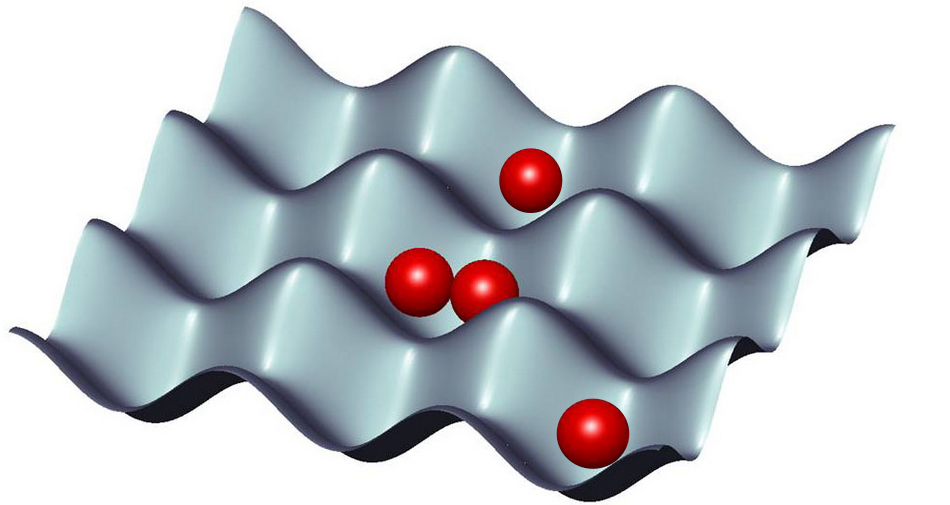
\includegraphics[width=8cm]{bosons_on_lattice}
    \end{center}
    \caption{Bosons on a 2D optical lattice. Figure is taken from\newline
             \texttt{www.uibk.ac.at/th-physik/qo/research/opticallattices.html.en}
            }
\end{figure}
There are further advantages which can make conducting experiments with
ultracold bosons on optical lattices more attractive than working with solids
directly. One is that there are always impurities present in the solids we find
in nature. These impurities can have significant impacts on the properties of
the solid which cannot necessarily be accounted for by a perturbative approach
which assumes these effects to be small. \todo{reference this at some point from
the book I meant to get from David}Optical lattices are highly uniform, so when
dealing with bosons on optical lattices this problem of impurities does not
arise.

Another benefit of working with bosons on optical lattices is that we can easily
control the state of each of the particles on the lattice. Furthermore, the
potential can be altered or switched off entirely during the experiment, which
is a feature that is not available in any solid state experiment
\cite{Morsch2006}.


\section{First quantised representation}

This paper will deal exclusively with bosons on optical lattices, and not
investigate cases involving fermions. There are a number of different
contributions to the Hamiltonian for bosons on optical lattices, and these
contributions can be seen to have analogues in condensed matter systems. The
individual bosons will have kinetic energy, and the potential created by the
lattice also contributes to how the system evolves in time, so it must feature
in the Hamiltonian. The bosons may be interacting, and there may also be an
external potential imposed that can vary in strength from site to site.

With regards to the interparticle interactions, we consider repulsive scattering
interactions. We will consider systems that are dilute, in the sense that the
average spacing between bosons is much greater than the effective range of the
interparticle interactions. This makes it reasonable to consider only
two-particle scattering events and neglect the rare higher order collisions,
provided we keep the strength of the interparticle interactions small. Even when
reduced to its two-body form, $U(x,x')$, the form of the interatomic scattering
potential has short range terms that can be difficult to deal with. We can
replace this object with a mathematically more convenient effective potential,
corresponding to contact interaction, with the same scattering cross-section at
low-energy. Because the ultracold bosons have such low energy, $s$-wave
scattering dominates, and the interparticle interaction potential can be
expressed simply in terms of the $s$-wave scattering length, $a_{s}$, as
\begin{equation}
    U_{\text{eff}}
    =
    \frac{2 \pi\hbar^{2} a_{s}}{m}
    \sum_{i,j}{\delta(x_{i} - x_{j})}.
\end{equation}
For simplicity, we will introduce the notation $U_{0} = \frac{4 \pi \hbar^{2}
a_{s}}{m}$. Having made these simplifications, we can construct a first
quantised Hamiltonian for a one-dimensional system of interacting bosons on an
optical lattice, in the presence of an external potential $V_{\text{ext}}$
\begin{equation}
    \label{eq:HamiltonianCoordinateRepresentation}
    \hat{h}
    =
    \sum_{i}{-\frac{\hbar^{2}}{2m}  \partial_{x_{i}}^{2}} +
    \sum_{i}{V_{\text{lattice}}(R_{i})} +
    V_{\text{ext}}(x) +
    \frac{U_{0}}{2} \sum_{i,j}{\delta(x_{i} - x_{j})}.
\end{equation}
Similar Hamiltonians are frequently used to describe systems of electrons on
atomic lattices. To promote conciseness, we introduce the abbreviations
\begin{equation*}
    \hat{h}_{1}
    =
    \sum_{i}{-\frac{\hbar^{2}}{2m} \partial_{x_{i}}^{2}} +
    \sum_{i}{V_{\text{lattice}}(R_{i})},
    \quad
    \hat{h}_{\text{ext}}
    =
    V_{\text{ext}}(x),
    \quad
    \hat{h}_{\text{int}}
    =
    \frac{U_{0}}{2} \sum_{i,j}\delta{(x_{i}-x_{j})}
\end{equation*}
so that $\hat{h}=\hat{h}_1+\hat{h}_{\text{ext}}+\hat{h}_{\text{int}}$.


\section{Effect of indistinguishability}
The Hamiltonian in the previous section would act on a bosonic many-particle wave function. A single particle wave function $\psi(\vec{r})$ is
defined within a Hilbert space $\mathcal{H}$, which is the space of complex, square integrable functions. It must satisfy $\int d^3\vec{r}|\psi(\vec{r})|^2<\infty$.
A wave function that represents the state of $N$ indistinguishable particles, $\psi(\vec{r}_{1},\vec{r}_{2},\dots,\vec{r}_{N})$ is defined within $\mathcal{H}^N$, where
$\mathcal{H}^N$ is constructed as the tensor product $N$ single-particle Hilbert spaces:
\begin{equation}
 \mathcal{H}^N=\mathcal{H}\otimes \mathcal{H} \otimes \dots\otimes \mathcal{H}.
\end{equation}
The wave functions in this space are also subject to normalisation constraints, i.e.,

\begin{equation*}
    \int d^{3} \vec{r}_{1} d^{3}\vec{r}_{2} \dots d^{3}\vec{r}_{N}
        \abs{\psi(\vec{r}_{1},\vec{r}_{2},\dots,\vec{r}_{N})}^{2}
    < \infty.
\end{equation*}
Whilst all functions satisfying the above constraints can be legitimately
defined mathematically, only a small subset are found to occur in nature --
those which are either entirely symmetric or anti-symmetric under particle
exchange. The set of indistinguishable particles which are entirely symmetric
under particle exchange are called bosons. This project will not investigate
scenarios involving the particles that display exchange anti-symmetry
(fermions), so we will be working within the space $S_{N}\mathcal{H}^{N}$. Here
$S_{N}$ projects onto the subspace of square-integrable functions that are
unchanged by permuting the order of the variables. As an illuminating example
one may construct the two-particle space, $S_{2}\mathcal{H}^{2}$ for bosons
as
\begin{equation*}
    S_{2} \mathcal{H}^{2}
    =
    \left \lbrace
        \psi \mid \psi = \psi_{1} \otimes \psi_{2} + \psi_{2} \otimes \psi_{1},
        \quad \text{where }\, \psi_{1}, \psi_{2} \in \mathcal{H}
    \right \rbrace
\end{equation*}
It is apparent that $S_{2} \mathcal{H}^{2} \ne \mathcal{H} \otimes \mathcal{H}$
since in this case we would be able to distinguish particles or states.
We can formally extend this notion of exchange symmetry for larger systems and
express the requirement of exchange symmetry for bosonic systems as
\cite{Negele1988}
\begin{equation*}
    \psi({\vec{r}_{\mathcal{P}_1}, \vec{r}_{\mathcal{P}_2}, \dots,
          \vec{r}_{\mathcal{P}_N}})
    =
    \psi(\vec{r}_{1}, \vec{r}_{2}, \dots, \vec{r}_{N}),
\end{equation*}
where $\lbrace \mathcal{P}_{1}, \mathcal{P}_{2}, \dots, \mathcal{P}_{N} \rbrace$
represents any permutation, $\mathcal{P}$, of the set $\lbrace 1, 2, \dots, N
\rbrace$.

Let us first consider the case of two indistinguishable bosons. We have not yet
determined the energy eigenstates of our Hamiltonian, but if we suppose we have
the set of normalised single-particle wave functions $\lbrace \ket{\lambda}
\rbrace$, and we have one boson in state $\ket{\lambda_1}$ and another in state
$\ket{\lambda_2}$, then we can write the two-particle wave function as
\begin{equation}
    \psi(\vec{r}_{1},\vec{r}_{2})
    =
    \frac{1}{\sqrt{2}}
    \big (
        \braket{\vec{r}_{1} | \lambda_1} \braket{\vec{r}_{2} | \lambda_2} +
        \braket{\vec{r}_{1} | \lambda_2} \braket{\vec{r}_{2} | \lambda_1}
    \big ),
\end{equation}
or in Dirac bra-ket notation, the two-body states would be represented as
\begin{equation}
    \ket{\lambda_1, \lambda_2}
    =
    \frac{1}{\sqrt{2}}
    \big (
        \ket{\lambda_1} \otimes \ket{\lambda_2} +
        \ket{\lambda_2} \otimes \ket{\lambda_1}
    \big ).
\end{equation}

The number of permutations that one must account for grows extremely quickly as
particle number increases. A properly symmetrised and normalised $N$-body state
can be represented \cite{Altland2010} as
\begin{equation}
    \ket{\lambda_{1}, \lambda_{2}, \dots, \lambda_{N}}
    =
    \frac{1}{\sqrt{N! \prod_{\lambda = 0}^{\infty}{n_{\lambda}}}}
    \sum_{\mathcal{P}}
        \ket{\lambda_{\mathcal{P}_{1}}} \otimes
        \ket{\lambda_{\mathcal{P}_{2}}} \otimes
        \dots                         \otimes
        \ket{\lambda_{\mathcal{P}_{N}}},
\end{equation}
where $n_{\lambda}$ is the number of particles in state $\lambda$, and the
summation runs over all $N!$ permutations $\mathcal{P}$ of the set of quantum
numbers $\lbrace \lambda_{1}, \dots, \lambda_{N} \rbrace$.

This formalism has a number of shortcomings. The most important of these for
this project is that it is extremely cumbersome for practical computation
because of the large number of entities that need to be represented. To avoid
this, we shall adopt the second quantised formalism, which is much better suited
to dealing concisely with large numbers of indistinguishable particles.
\newpage


\section{Second Quantisation}

\subsection{The Occupation Number Representation}

The formalism that we have hitherto discussed explicitly represents a
significant amount of redundant information, in the sense that it deals
separately with the scenarios ``particle 1 in state $\lambda_1$ and particle 2
in state $\lambda_2$'' and ``particle 2 in state $\lambda_1$ and particle 1 in
state $\lambda_2$''. Taking into account the indistinguishability of the
particles, it is clear that these two scenarios are identical. A more efficient
approach consists of describing the number of particles in a particular state
$\lambda_i$, i.e., using the occupation number representation. When doing this,
a general state can be written as a linear superposition
\begin{equation}
    \ket{\Psi}
    =
    \sum_{n_{1}, n_{2}, \dots}%
        {c_{n_{1}, n_{2}, \dots}\ket{n_{1}, n_{2}, \dots}}.
\end{equation}
In the scenario which this project will be working with, the occupation numbers
refer to the number of bosons on a particular site of the lattice. Having
established this, we can define creation and annihilation operators that create
and annihilate particles from number eigenstates, that is
\begin{equation}
    \hat{a}_{j}^{\dagger} \ket{n_{1}, n_{2}, \dots, n_{j}, \dots}
    =
    \sqrt{n_{j} + 1} \ket{n_{1}, n_{2}, \dots, n_{j}+1, \dots}
\end{equation}
and
\begin{equation}
    \hat{a}_{j} \ket{n_{1}, n_{2}, \dots, n_{j}, \dots}
    =
    \sqrt{n_{j}} \ket{n_{1}, n_{2}, \dots, n_{j}-1, \dots}.
\end{equation}
These operators have very important commutation relations
\begin{equation}
    [ \hat{a}_{j}^{\dagger}, \hat{a}_{k}^{\dagger}] = 0, \quad
    [ \hat{a}_{j}, \hat{a}_{k}]=0, \quad
    [\hat{a}_{j},\hat{a}_{k}^{\dagger}]=\delta_{jk}.
\end{equation}
We can also define the number operator $hat{n}_{j} = \hat{a}_{j}^{\dagger}
\hat{a}_{j}$ that has the property that
\begin{equation}
    \hat{n}_{j} \ket{n_{1}, n_{2}, \dots, n_{j}, \dots}
    =
    n_{j} \ket{n_{1}, n_{2}, \dots, n_{j}, \dots}.
\end{equation}

The occupation number eigenstates form the basis of the $N$-particle Hilbert
space that we are working in (the Fock space $\mathcal{F}^N$), and it is useful
to observe that any occupation number eigenstate can be created from the empty
(or ``vacuum'') state $\ket{0}$ by repeated action of
creation operators \cite{Altland2010}
\begin{equation}
 \ket{n_1,n_2,\dots}=\prod_i\frac{1}{\sqrt{n_i!}}(\hat{a}_i^{\dagger})^{n_i}\ket{0}.
\end{equation}

It may seem that the state space $S_N\mathcal{H}^N$ that we have constructed is
not robust enough to accommodate these operators. Indeed, the creation and
annihilation operators take us from the $N$-particle Hilbert space to the
$(N+1)$- and $(N-1)$-particle Hilbert spaces, respectively. In order to account
for these differences in particle number, we must really be working within the
symmetric Fock states $\mathcal{F}_{S}(\mathcal{H})$, defined by the direct sum
\cite{Blank1999}
\begin{equation}
    \mathcal{F}_{S}(\mathcal{H}) = \oplus_{N=0}^\infty S_{N} \mathcal{H}^N.
\end{equation}

However, we will be working in systems in which the particle number is
conserved. Each combination of creation and annihilation operators that appears
in the Hamiltonian will create an equal number of particles to the number
destroyed. So for practical purposes we are just working within $S_{N}
\mathcal{H}^{N}$.

Having established the space and states that we are operating with, we now need
to rewrite the Hamiltonian in number state representation, i.e., we need to
``second quantise'' it.


\subsection{Second Quantisation of the Hamiltonian}

We can second quantise the Hamiltonian initially used to describe our system
through the boson field operators, $\hat{\psi}^{\dagger}(x)$ and
$\hat{\psi}(x)$, which create and destroy particles at particular spatial
locations (we will define these more explicitly later). The two terms in
$\hat{h}_1$ are single-particle operators for the kinetic and potential energy
contributions, and can be transformed to
\begin{equation}
    \hat{H}_{1}
    =
    \int{\hat{\psi}^{\dagger}(x) \hat{h}_{1} \hat{\psi}(x) \,dx}.
\end{equation}

The one-dimensional Bloch's theorem states \cite{Bloch1929, Kittel1987} that the
eigenstates of a particle in a periodic potential have the form
\begin{equation}
    \phi_{q}(x) = e^{iqx} u_{q}(x),
\end{equation}
where $q$ is the quasi-momentum and $u_{q}(x)$ is periodic with the same period
as the lattice, $d$. We will be considering scenarios in which the strength of
the lattice potential is such that the bosons are not completely localised, but
such that the overlap between the wave functions of particles on particular
lattice sites have effectively zero overlap with non-nearest neighbours. Under
these conditions, the wave functions can be conveniently described by the
localised Wannier functions
\begin{equation}
    \psi(R;r) = \frac{1}{d} \int{dq\, e^{iRq} \phi_{q}(x)}
\end{equation}
which are superposition of Bloch functions \cite{Kittel1987, Wannier1937}. This
is a useful description because the Wannier functions are both orthonormal and,
more importantly, complete. We can use this to rewrite the field operators as
\begin{equation}
    \label{field_operators_wannier}
    \hat{\psi} = \sum_{j}{\hat{a}_{j}\psi(R_{j} - x)}.
\end{equation}
\todo{Time-dependence in $a$?}
With this in mind, we can write
\begin{equation}
    \int{
         \sum_{j}{\hat{a}_j^{\dagger}\psi^{*}(R_j-x)}
         \hat{h}_{1}
         \sum_{l}{\hat{a}_l\psi(R_{l} - x)}
         \,dx}
    =
    \sum_{j,l}{J_{j,l} \hat{a}_{j}^{\dagger} \hat{a}_{l}}.
\end{equation}
Here we have introduced a shorthand notation
\begin{equation}
 J_{j,l} = \int{\psi^{*}(R_{j} - x) \hat{h}_{1} \psi(R_{l}-x) \,dx}
\end{equation}
for the numerical values of these integrals. Notice that the integration --at
least numerically-- can indeed be carried out and characterises the strength of
the hopping between sites $j$ and $l$. It is typically described \todo{need
references!} as characterising the overlap of the single-particle spatial wave
functions (see figure below).
\begin{figure}[h!]
    \begin{center}
        \includegraphics[width=0.8\textwidth]{J_overlap_drawing}
    \end{center}
    \caption{\label{fig:J_overlap_drawing}
             The strength of hopping $J$ is considered as the overlap of
             localised Wannier functions centred at neighbouring lattice sites.}
\end{figure}
This is not entirely accurate, as the Wannier states are orthonormal and so the
integral over their inner product is zero. More precisely, $J_{j,l}$ takes the
inner product between a Wannier state $\psi(R_{j} - x)$ and the state produced
by the action of $\hat{h}_1$ on the Wannier state $\psi(R_{l} - x)$, which does
not have to be zero. However, the depiction in figure \ref{fig:J_overlap_drawing}
can still be useful for developing an intuition for what $J$ is, since $J$
depends on the combination of the lattice depth (and width) and the kinetic
energy and so would the overlap of the spatial wave functions if they were not
orthonormal. It is also clear from the figure that computing overlap integrals
using wave functions on non-neighbouring sites does not add much accuracy to our
model, so we neglect these. For the hopping interactions that are permitted, we
assume that each has identical strength. This assumption allows us to write
\begin{equation}
    \hat{H}_{1}
    =
    \int{\hat{\psi}^{\dagger}(x)
         \bigg(
            \!\sum_{i}{-\frac{\hbar^{2}}{2m} \partial_{x_{i}}^{2}} +
            \sum_{j}{V_{\text{lattice}}(R_{j})}
         \bigg)
         \hat{\psi}(x) \,dx}
    =
    J \sum_{i}{(\hat{a}^\dagger_{i}\hat{a}_{i+1}+h.c.)},
\end{equation}
where $h.c.$ denotes the hermitian conjugate. We can go through a similar
process for the contributions of the external potential and on-site interactions
between bosons. The external potential gives an on-site energy that can vary at
different locations in the lattice
\begin{equation}
    \hat{H}_{\text{ext}}
    =
    \int{\hat{\psi}^{\dagger}(x) V_{\text{ext}}(x) \hat{\psi}(x) \,dx}
    =
    \sum_{i}{\epsilon_{i} \hat{a}_{i}^{\dagger} \hat{a}_{i}}.
\end{equation}

The term for on-site interaction between bosons is a two-particle operator, thus
second quantisation requires integration between two sets of boson field
operators
\begin{equation}
    \hat{H}_{\text{int}} =
    \int{\hat{\psi}^{\dagger}(x) \hat{\psi}^{\dagger}(x)
          \frac{U_{0}}{2} \sum_{i,j}{\delta(x_{i}-x_{j})}
          \hat{\psi}(x) \hat{\psi}(x) dx
        }
    =
    \frac{U_{0}}{2}
    \sum_{i}
        {\hat{a}_{i}^{\dagger} \hat{a}_{i}^{\dagger} \hat{a}_{i} \hat{a}_{i}}
\end{equation}

Putting these terms together, we arrive at the Bose-Hubbard model described in
the next section.


\section{The Bose-Hubbard model}

The Hamiltonian for a weakly interacting BEC in a one-dimensional optical
lattice and subject to harmonic trapping potential is given by the sum of
$\hat{H}_{1}$, $\hat{H}_{\text{ext}}$ and $\hat{H}_{\text{int}}$:
\begin{equation}
    \hat{H}_{\text{1D}}
    =
    J \sum_{i}{(\hat{a}^\dagger_{i}\hat{a}_{i+1} + h.c.)} +
    \frac{U_{0}}{2}
    \sum_{i}%
        {\hat{a}_{i}^{\dagger} \hat{a}_{i}^{\dagger} \hat{a}_{i} \hat{a}_{i}} +
    \sum_{i}%
        {\epsilon_{i} \hat{a}_{j}^{\dagger} \hat{a}_{j}},
\end{equation}
and is known as the Bose-Hubbard Hamiltonian. The $\epsilon_{i}$'s refer to
on-site energies at each lattice site due to the harmonic trap, and the middle
term gives an interaction energy when there is more than one particle on a
particular site. This project will look at scenarios where there is no external
harmonic potential which produces different on-site energies for different sites
(the uniform lattice potential remains, so $J$ is still defined as before). In
the absence of this external potential, the Hamiltonian in one dimension reduces
to
\begin{equation}
\begin{align*}
\hat{H}_{1D}=&J\sum_{i}(\hat{a}^\dagger_{i}\hat{a}_{i+1}+h.c.\ ) +\frac{U_0}{2}\sum_{i}\hat{a}^\dagger_{i}\hat{a}^\dagger_{i}\hat{a}_{i}\hat{a}_{i}.
\end{align*}
\end{equation}

This project aims to explore the dynamics of both this one dimensional system and the two dimensional version where we couple multiple chains of lattice sites together. The
system Hamiltonian in two dimensions is

\begin{equation}
\hat{H}_{2D}=(J\sum_{i,j}\hat{a}^\dagger_{i,j+1}\hat{a}_{i,j} + J'\sum_{i,j}\hat{a}^\dagger_{i,j}\hat{a}_{i+1,j})+h.c. +\frac{U_0}{2}\sum_{i}\hat{a}^\dagger_{i}\hat{a}^\dagger_{i}\hat{a}_{i}\hat{a}_{i},
\end{equation}
where the $i$ index denotes which chain is being referred to and the $j$ index denotes how far along the chain a site is. $J'$ is another hopping parameter; it characterises the
overlap between adjacent Wannier states \todo{factcheck: should this be Bloch states? or neither?}on different chains.
\begin{figure}[H]
    \begin{center}
        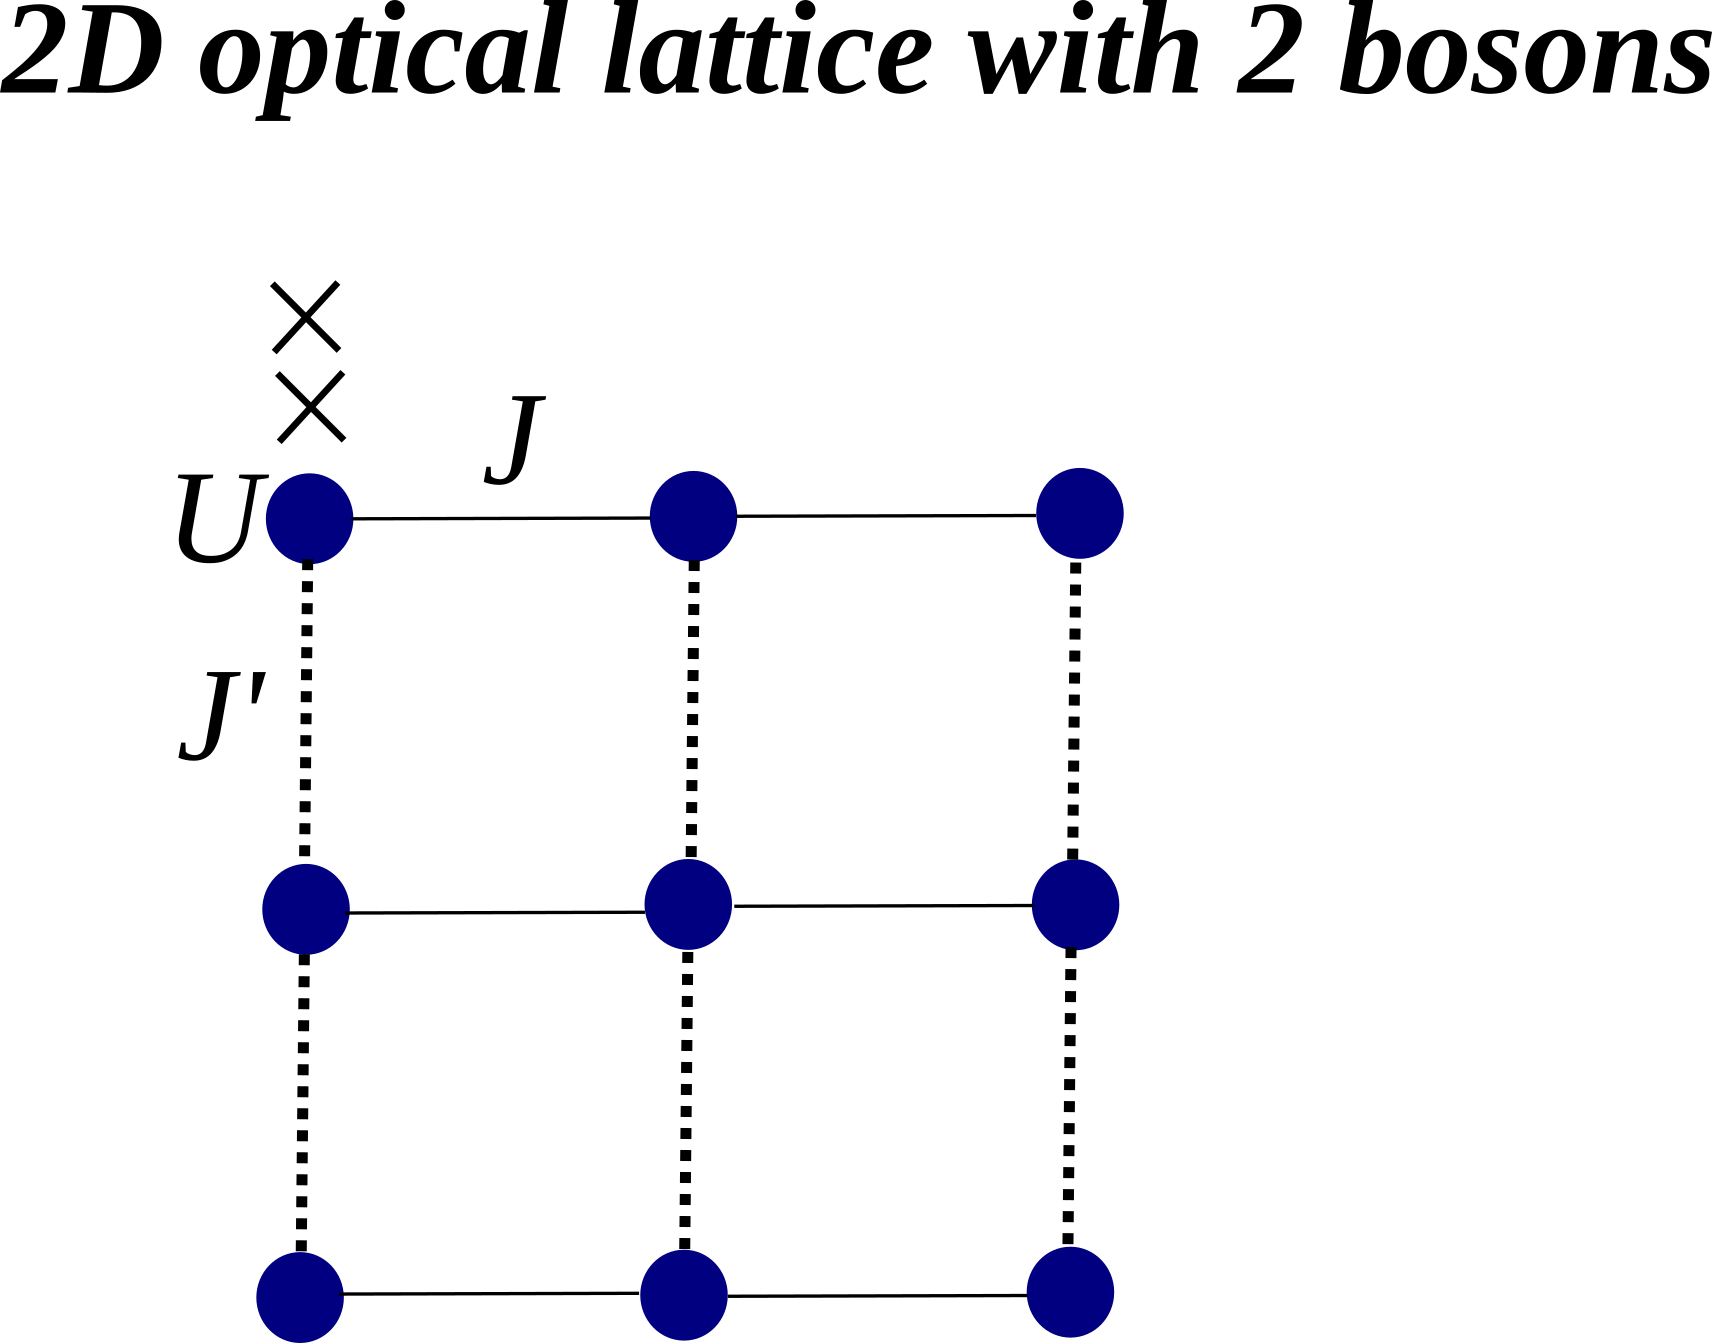
\includegraphics[width=8cm]{lattice_pic}
    \end{center}
    \caption{The blue circles here represent lattice sites and the crosses
             denote individual bosons. Hopping between any two neighbouring
             sites on the same chain is characterised by $J$, whereas hopping
             between chains is characterised by $J'$. A three by three lattice
             is shown here, but the system can be extended to arbitrary size.
            }
\end{figure}
We are interested in the time evolution of these systems as it relates to their
thermal behaviour.


\section{Thermalisation}
 \subsection{Overview}

Thermalisation refers to a relaxation of a system to states where the values of macroscopic quantities are stationary, universal with respect to
widely differing initial conditions, and predictable using statistical mechanics \cite{Rigol2008}. We observe thermalisation in a wide variety of classical systems, and there
are strong theoretical reasons for anticipating this thermalisation. However, many of these reasons don't apply when considering quantum systems. The question of
which, if any, quantum systems exhibit thermalisation and how the thermal states can be characterised is of considerable theoretical and experimental interest.

 \subsection{Classical systems}
To see why thermalisation is common and even expected in many classical systems, we need to understand the property of ergodicity and the impact of chaotic dynamics on it.
If you start an isolated system in a particular configuration corresponding to a particular point in phase space, it can move through that phase space along the constant-energy
manifold. A system is ergodic if the long-term time average of any single phase space trajectory is equivalent to an ensemble average. \todo{get Kinoshita's definition of ergodicity}
\todo{Do I need to elaborate on this further?}Classical systems \todo{often? usually? sometimes?} exhibit chaotic dynamics, which are strongly nonlinear and allow the system to quickly
and essentially uniformly explore the constant-energy manifold irrespective of the initial conditions. This promotes ergodicity, which is implicit in the fundamental assumption of
statistical mechanics - all accessible microstates are equiprobable. \todo{Need to explicitly link ergodicity and thermalisation, otherwise this is just free-floating and its
relevance is not obvious. What is this link?} This is what leads us to expect our classical systems to thermalise.

 \subsection{Quantum systems}
Quantum systems do not \todo{usually?} exhibit dynamic chaos \todo{see square brackets} [Rigol's line is ``dynamical chaos itself cannot occur in an isolated quantum system, in which the time
evolution is linear and the spectrum is discrete'' How does that argument work?], so it is not obvious how one would justify applying the assumption of ergodicity in these systems. Because of
this, it is unclear if, or when, we should expect quantum systems to thermalise, or what statistical ensemble we could use to characterise the relaxed states.


\section{Integrable systems}
There are a number of classical, isolated systems that do not display thermalisation. The main difference between these systems and those which approach thermal equilibrium is the extent to which
they are constrained relative to the number of degrees of freedom that they posess. This observation is formalised in the notion of integrability. A system is said to be integrable if it has \todo{half? according to
handout this seems to be the case} as
many independent integrals of motion (which are conserved) as it has degrees of freedom. An integral of motion for a Hamiltonian is a smooth function $I$ defined on an open subset of the
phase space such that $\dot{I}=0$ on solutions. \todo{reference handout Danny gave me, I can't see anywhere where its from}So $I(x(t))=\text{constant}$, where $x(t)$ is the solution of the equations of motion
for a particular initial condition. If $x_1(t)$ and $x_2(t)$ are solutions for different initial conditions, then in most cases $I(x_1(t))\ne I(x_2(t))$.
Integrability is a useful property, though it is quite rare.

Theoretically, we can find exact solutions for the equations of motion for a system if it is integrable, otherwise we cannot.
In classical mechanics, the idea of integrability is well-understood and neatly defined. The situation in quantum mechanics is much more challenging. One reason for this is that
the Heisenberg uncertainty principle prevents us from applying the idea of points in phase space with particular trajectories.

With respect to the systems that we are dealing with, it has been shown that a one-dimensional lattice chain of non-interacting bosons is an integrable system \cite{Rigol2007}.



\todo{see square brackets} [Maybe fall back on ``All 1D systems with conserved energy are integrable'' for U!=0, referencing page 6 of the handout Danny gave me. I don't really know where
to go for 2D at this point.]

\newpage
\section{Experimental studies}
\subsection{A quantum Newton's cradle}
Kinoshita et. al. investigated \cite{Kinoshita2006} the thermalisation of an out-of-equilibrium 1D Bose gas, which is a  nearly-integrable system. They started with
several thousand arrays of one-dimensional Bose gases, each containing from $40$ to $250$ $^{87}$Rb atoms. The atoms were trapped by combining a blue-detuned \todo{check I understand why this one is
blue-detuned and the other red-detuned} two dimensional optical lattice, which provides tight transverse confinement, with a red-detuned crossed dipole trap \todo{what is a crossed dipole trap?}
providing weak axial trapping. In order to create the non-equilibrium momentum distributions, they then pulsed on a $3.2$ THz detuned 1D lattice, which depletesd the zero momentum state
and put the atoms in a superposition momentum state of $\pm2\hbar k$. The two parts of the wave function then oscillated out of phase with each other, colliding with each other twice every full cycle
and either reflecting off each other elastically or transmitting straight through like a ``ghostly'' Newton's cradle (see diagram below)

\begin{figure}[H]
 \begin{center}
 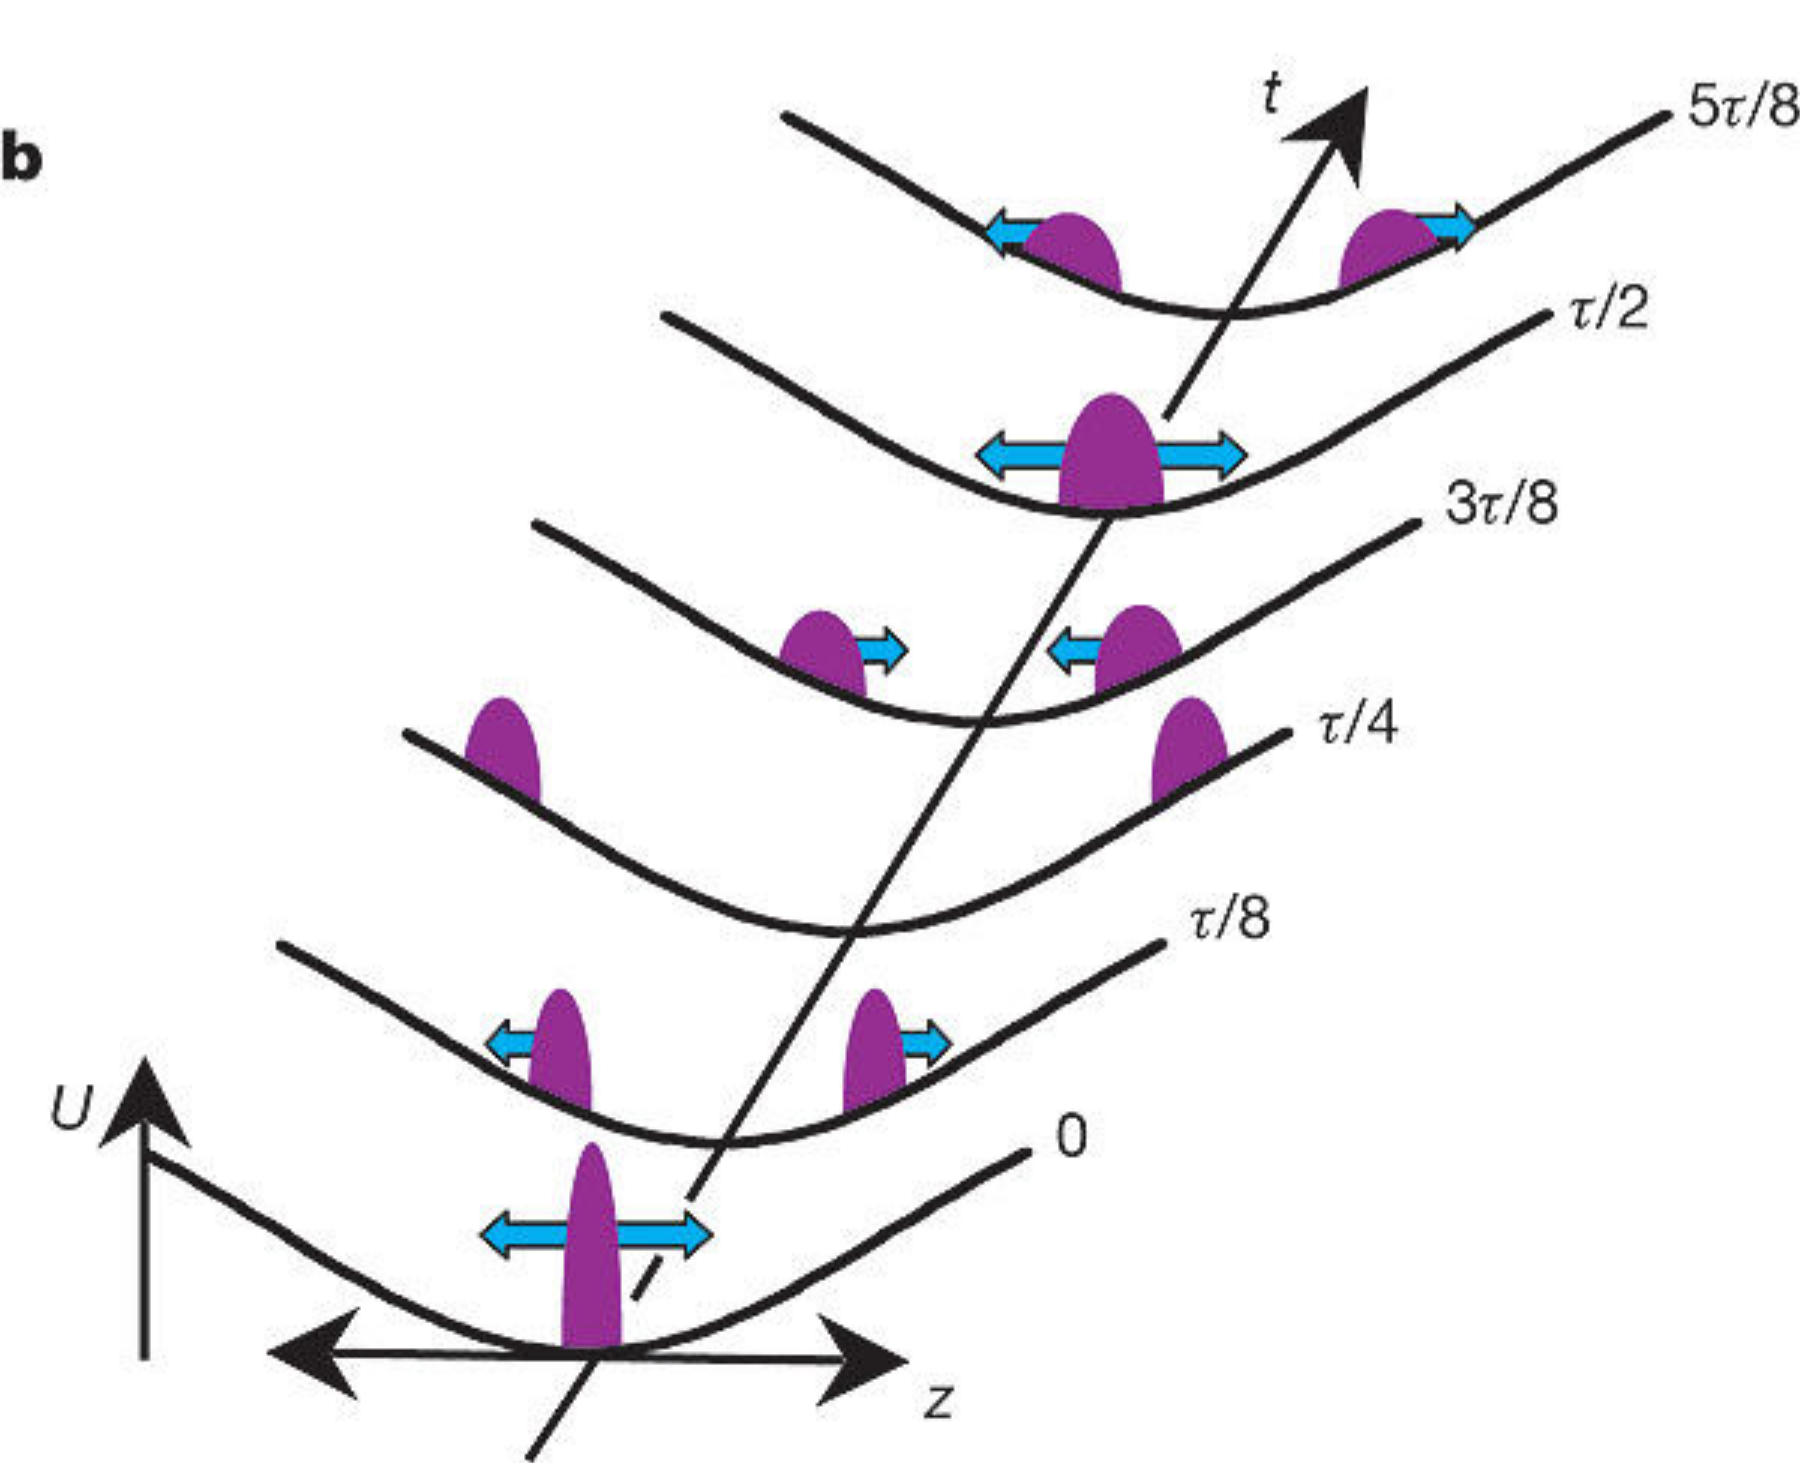
\includegraphics[width=8cm]{quantum_newtons_cradle}
 \end{center}
 \caption{Sketches at various times of two out of equilibrium
clouds of atoms in a 1D anharmonic trap. At time $t=0$ the atoms are put into a momentum superposition with $2\hbar k$ to the right and $2\hbar k$ to the left. The two parts of the
wave function oscillate out of phase with each other with a period $\tau$. Each atom collides with the opposite momentum group
twice every full cycle, for instance, at $t=0$ and $t=\frac{\tau}{2}$. Figure is from reference \cite{Kinoshita2006}.}
 \end{figure}

The weak anharmonicity of the trap caused the atoms to gradually dephase. However, the momentum distribution after dephasing was not gaussian (as one would expect for a thermalised state),
and this momentum did not noticeably tend toward this equilibrium distribution, even after thousands of collisions.

\begin{figure}[H]
 \begin{center}
 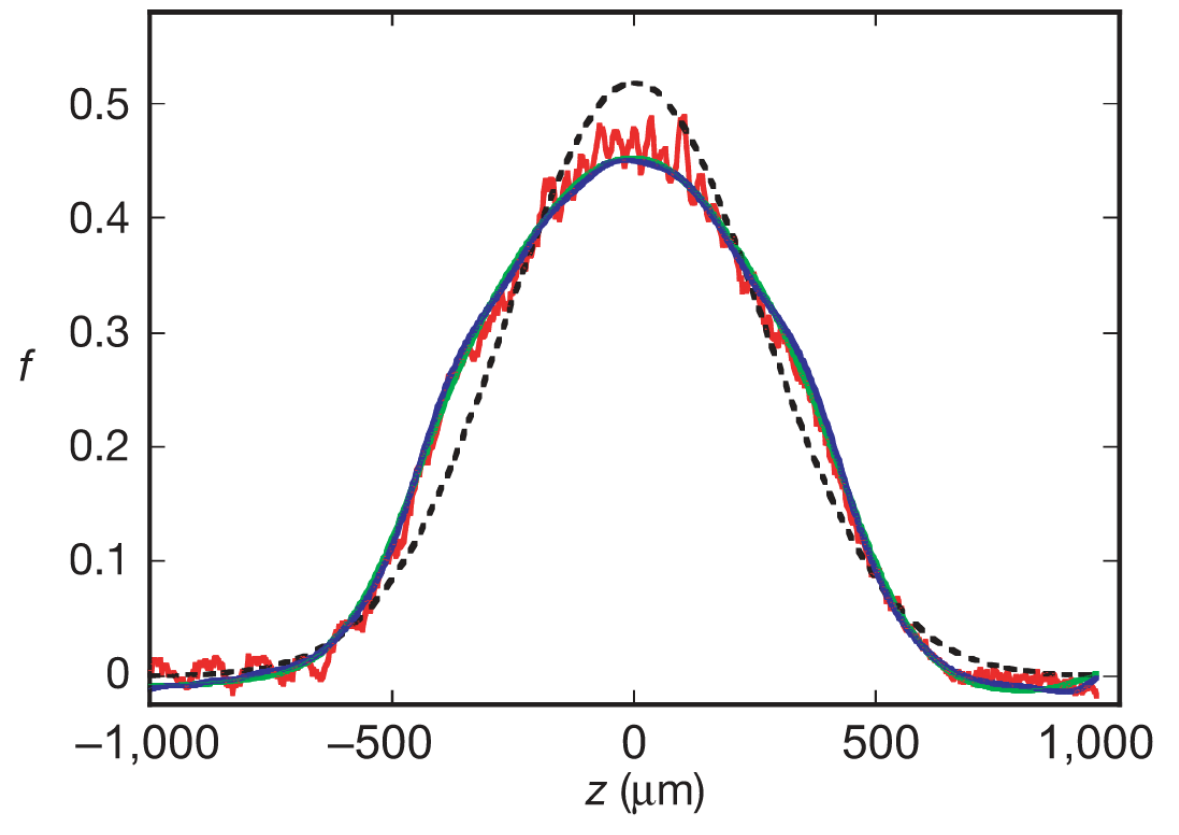
\includegraphics[width=1.0\textwidth]{dephased_momentum_distribution}
 \end{center}
 \caption{\label{dephased_momentum_distribution}The blue and green curves in the above figure are projections from models that take into account loss and heating. The red line is the actual distribution observed. The dashed line
 is a gaussian with the same number of atoms and r.m.s. width as the actual distribution. }
 \end{figure}


To the extent that the actual distribution in figure \ref{dephased_momentum_distribution} conforms to the projected distribution rather than to the gaussian, the atoms have not
thermalized.

These observations extended from the Tonks--Girardeau regime, which has very strong repulsive interactions between bosons so only pairwise collisions can occur, to the intermediate
coupling regime, where there can be three- (or more) body collisions.
\newpage
\subsection{Relaxation in a Completely Integrable Many-Body Quantum System}

Inspired by the ``A Quantum Newton's Cradle'' study, investigations were made into a completely integrable many-body quantum system. In this experiment, hard-core bosons \todo{find a good
description of what makes bosons "hard core``} on a 1D lattice were used. The authors, Rigol et. al \cite{Rigol2007}, started with a one dimensional bosonic Hamiltonian with no interactions
and periodic boundary conditions for a lattice with $L$ lattice sites.
\begin{equation}
 \hat{H}=-J\sum_{i=1}^{L} (\hat{a}_{i}^{\dagger}\hat{a}_{i+1}+h.c.)
\end{equation}

They then mapped their bosonic system to a free ferminonic one using a Jordan-Wigner transformation:
\begin{equation}
 \hat{H}=-J\sum_{i=1}^{L} (\hat{c}_{i}^{\dagger}\hat{c}_{i+1}+h.c.)
\end{equation}
Here $\hat{c}_{i}^{\dagger}$ and $\hat{c}_{i+1}$ are fermionic creation and annihilation operators.
The integrals of motion were the fermionic quasi-momentum distribution operators, and the system thus must be integrable because
there are as many of these operators as they had lattice sites. They have numerically investigated the time evolution of this system and found it to undergo relaxation to an equilibrium
state. The properties of the state that the system relaxed to were not given by the grand-canonical ensemble, but rather by a generalised Gibbs ensemble, in which the partition function
is extended to include all of the integrals of motion.


\begin{figure}[H]
 \begin{center}
 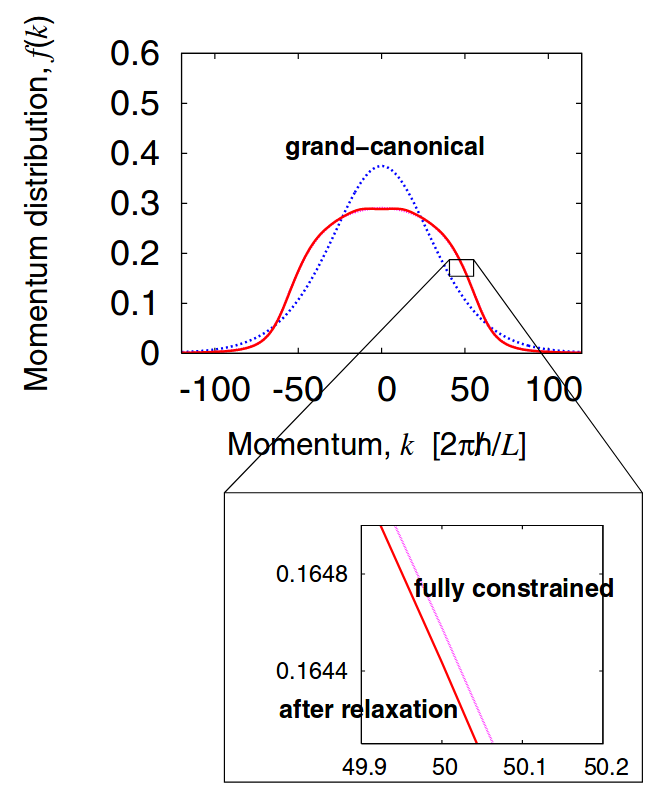
\includegraphics[width=8cm]{grand_canonical_vs_GGE}
 \end{center}
 \caption{Equilibrium (quasi-)momentum distribution after relaxation in comparison with the predictions of the grand-canonical and of
the fully constrained thermodynamical ensembles. The prediction  of the fully constrained  ensemble  is virtually  indistinct
from the results of the dynamical simulation. Image taken from \cite{Rigol2007}.}
 \end{figure}
\todo{the above caption (except the first sentence) is currently copy-pasted from the paper. I'm not sure how to reword those sentences any other way}


They further showed that their generalized equilibrium state carries more memory of the initial conditions than the usual thermodynamic one.

\begin{figure}[H]
 \begin{center}
 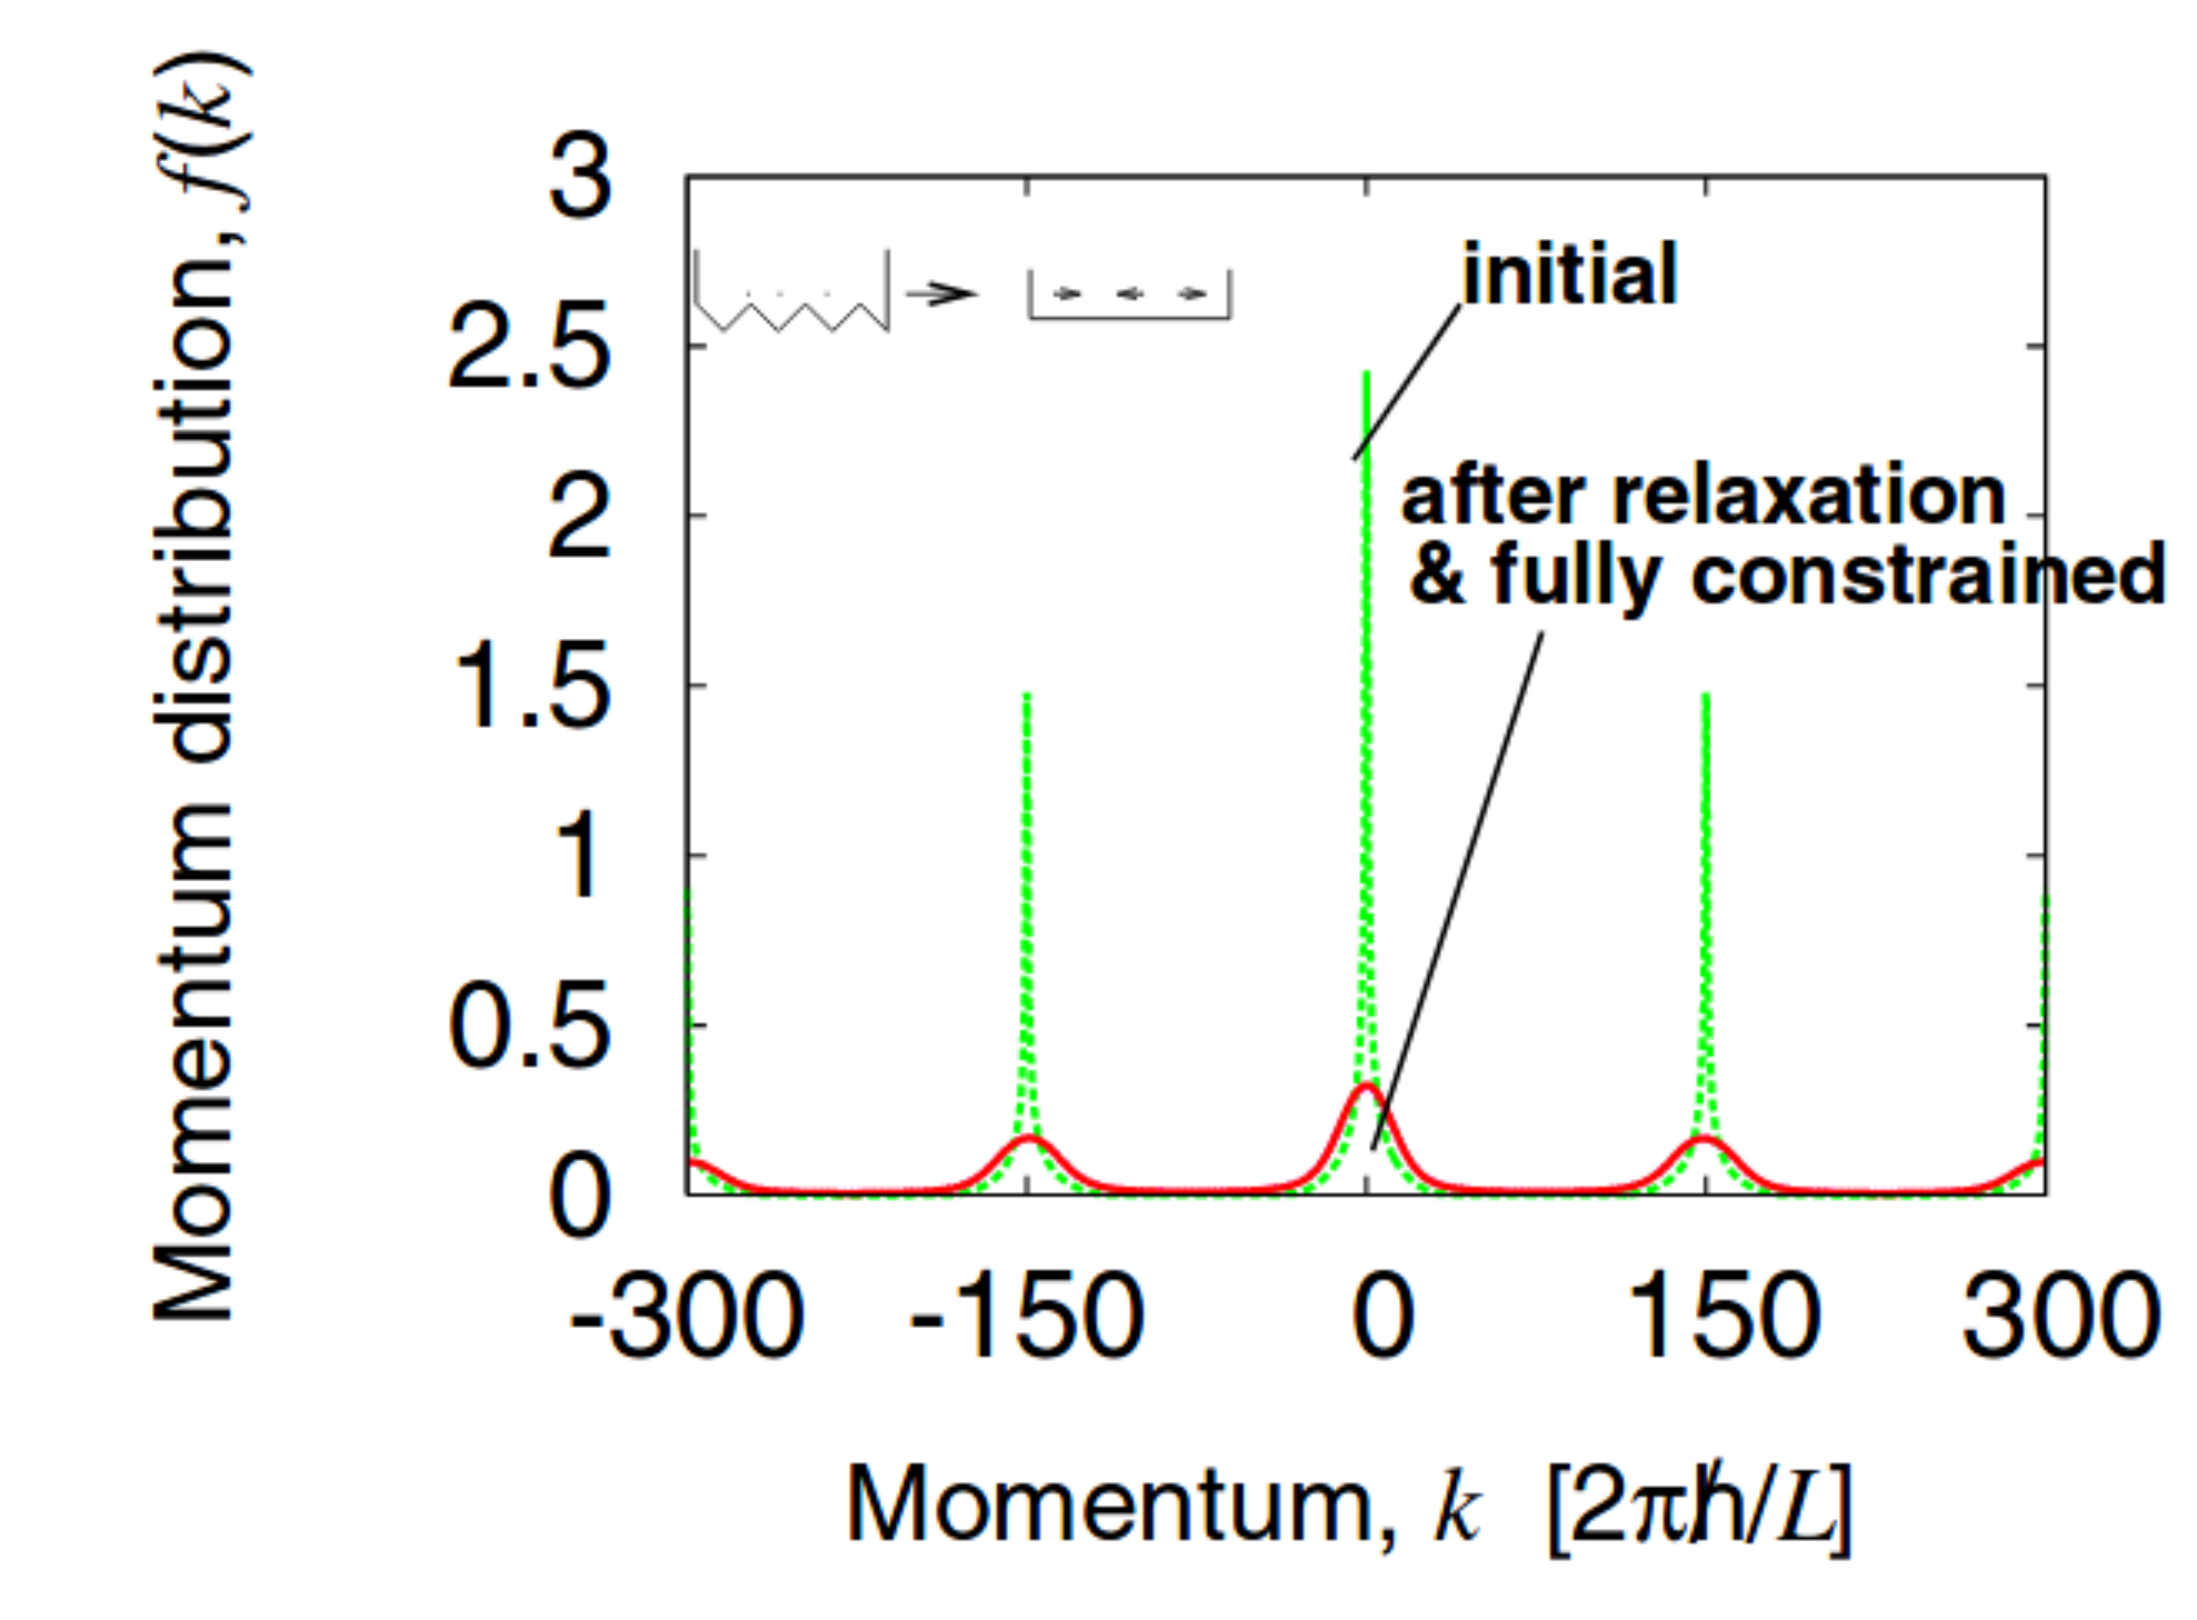
\includegraphics[width=8cm]{after_relaxation_rigol}
 \end{center}
 \caption{The actual quasi-momentum distribution after relaxation vs predictions of the generalised Gibbs ensemble and the grand canonical ensemble. Image taken from \cite{Rigol2007}.}
 \end{figure}

The momentum peaks remain clear and distinct during the whole duration  of  propagation; $t_{\text{fin}}=3000\hbar/J$.

\subsection{Measuring entanglement entropy in a quantum many-body system}
- I still don't see how this is supposed to relate to what I'm doing.
I can write down the definition of the nth order R\'enyi entropies, and describe what purity is.
I imagine that I could construct a system that is a 2 by N lattice and split it into two one-dimensional lattices of length N, then evaluate their purity (which must be zero for one of the
chains and 1 for the other if I'm starting with all bosons on one site, right?), then do some second order renyi entropy calculation based on that. Then I could evolve the system in time
and note that this entropy changes. How does that relate the thermalisation? What can I find out from this approach that I don't already get from just looking at expectation values of number
operators?

\newpage

\section{System size and analyticity}

Whilst the main focus of this project is on smaller lattices with few particles, it is of interest to investigate larger system sizes (necessarily by approximate methods) to see how much
of the behaviour of the small systems is preserved in the larger ones.

\subsection{Small systems}

We can decompose any time evolved state $\ket{\psi(t)}$ of our system in terms of its state at $t=0$, $\ket{\psi(0)}$, and the energy eigenvectors $\ket{E_n}$ (see section \ref{revival}
for details):
\begin{equation}
  \ket{\psi(t)}=\sum_je^{iE_{j}t}\ket{E_j}\braket{E_j|\psi(0)}.
\end{equation}
Calculating $\ket{\psi(t)}$ from the above formula requires that we diagonalise
the Hamiltonian and find its energy eigenvectors and eigenvalues. This is easy
for small systems, in particular those that have only a single particle on them.
This method has the significant advantage of being ``analytic'', at least up to
the precision of the values stored for the eigenvalues and eigenvectors. All
instances of $\ket{\psi(t)}$ are calculated from the initial state
$\ket{\psi(0)}$, so the value \todo{is value the right word since psi(t)
is a vector?}we calculate for $\ket{\psi(t)}$ is independent of the timestep
between each instance of $\ket{\psi(t)}$ that we calculate. This has the further
advantage that in a numerical algorithm we need not concern ourselves with
drifting of the norm\todo{clunky sentence}. However, as the number of lattice
sites and particles in the system increases, the time required to apply this
method increases dramatically. This is because the dimensionality $\mathcal{D}$
of the system grows according to
\begin{equation}
 \mathcal{D}=\frac{\left(N+P-1\right)!}{P!\left(N-1\right)!}, \label{time_evolution}
\end{equation}
where $N$ is the number of lattice sites and $P$ is the number of particles on the lattice. Unsurprisingly, this is the same as the number of possible pure number states (since these form
an orthonormal basis), and so the formula deduced is just the formula for the number of ways to arrange $P$ objects into $N$ containers that is familiar from elementary statistical mechanics.
The Hamiltonian is a $\mathcal{D}\times\mathcal{D}$ square matrix, and diagonalising it and then evolving the system according to equation (\ref{time_evolution}) quickly becomes impractical
for systems with large numbers of particles and lattice sites. For these systems, a different approach to time evolution is required. We have chosen to use a Gross-Pitaevskii equation to reduce
the dimensionality of the system. Doing this forces us to take an iterative approach to time evolution rather than an analytic one. A Runge-Kutta-Feldberg algorithm \cite{Burden2005} was written for this purpose.

\subsection{The Gross-Pitaevskii Equation (GPE)}
The GPE is a classical mean-field equation for describing Bose-Einstein condensates (BECs) in the zero-temperature limit. In the smaller systems that we consider with the analytic method, it is rare
for us to have more than two particles on a lattice, and hence the concept of ``macroscopic occupation of the ground state'' that is integral to Bose-Einstein condensation has little importance here.
The validity of some of the assumptions that we make in this method will rely on there being a large number of particles. \todo{keep going here with masters thesis info, what's another good source?}
When second quantising our Hamiltonian earlier, in equation \label{field_operators_wannier} we decomposed the field operators into linear combinations of single-particle Wannier position states.
However, it is possible to decompose the field operators into any complete single-particle basis. If we chose the single particle energy basis $\{\phi_i\}$, then we get
\begin{equation}
 \hat{\Psi}(\vec{r})=\sum_{i=0}^\infty \hat{a}_i\phi_{i}(\vec{r}) = \hat{a}_0\phi_{0}(\vec{r}) + \sum_{i=1}^\infty \hat{a}_i\phi_{i}(\vec{r}).
\end{equation}
Since the GPE is a tool for investigating near-zero temperature BECs (very low energy systems), we now assume that the occupancy of energy modes other than the ground modes is negligible, i.e.,
\begin{equation}
 \hat{\Psi}(\vec{r})=\hat{a}_0\phi_{0}(\vec{r}).
\end{equation}



\section{Results}

\section{Revival \label{revival}}

In a subset of the integrable systems considered, we observed regular instances in which the system would return to the state in which it was initially prepared (it ``revives'').
To see why we might expect to see revival in some cases, consider the initial state of the system $\ket{\psi(0)}$, which evolves in time according to
\begin{equation}
 \ket{\psi(t)}=e^{i\hat{H}t}\ket{\psi(0)}.
\end{equation}
Now noting that we can use the completeness relation for the energy eigenstates to expand the initial state in the energy basis,
and incorporating the $\hbar^{-1}$ into the time scale,
\begin{align}
 \ket{\psi(t)} =&       e^{i\hat{H}t}\sum_j\ket{E_j}\braket{E_j|\psi(0)}  \nonumber \\
               =&\sum_je^{i\hat{H}t}\ket{E_j}\braket{E_j|\psi(0)} \nonumber \\
                =&\sum_je^{iE_{j}t}\ket{E_j}\braket{E_j|\psi(0)}  \nonumber \\
                =&\sum_j c_{j}e^{iE_{j}t}\ket{E_j}
\end{align}

From here it can be seen that the only time dependence appears in the complex exponentials, each of which is $2\pi$-periodic. If we can find some common time $t_r$ such
that $E_{j} t_{r}=2 \pi k_{j}$, where $k_{j} \in \mathbb{Z} $ for all $j$, we will recover the initial state exactly, i.e., $\ket{\psi(t_{r})}=\ket{\psi(0)}$.
The next section describes the conditions necessary for the existence of the revival time.\\


\subsection{Exact revival}

We observe an exact and regular revival in precisely the cases in which the
eigenvalues are mutually rational, i.e. they are either all rational, or are all
rational when divided by the same irrational number.
\begin{definition}[Mutually rational set]
    We say that a set of eigenvalues are mutually rational if they are all
    rational when divided by a common real number.
\end{definition}




For example, the set of
hypothetical eigenvalues $\lbrace 0, \sqrt{2}, 2 \sqrt{2}, \frac{3 \sqrt{2}}{10}
\rbrace$ is mutually rational, whereas $\lbrace 0, \sqrt{2}, \sqrt{3}\rbrace$ is
not. In the case of mutually rational eigenvalues, we can write $E_{j} =
\frac{p_{j}}{q_{j}}$, where $p_{j}$, $q_{j} \in \mathbb{Z}$. The revival time is
then given by $t_{r} = 2\pi Q_{LCM}$, where $Q_{LCM}$ is the lowest common
multiple of ${q_j}$.

We are yet to find any systems with nonzero interparticle interaction that have
mutually rational eigenvalues. In one dimension, the only systems that we have
found that meet the criterion of mutually irrational eigenvalues are those with
fewer than 4 lattice sites. In two dimensions, \todo{do a comprehensive batch of
simulations to determine what is and isn't ok in 2D}.

To demonstrate this exact revival, consider a one dimensional lattice with three
sites with a single boson and hopping constant $J$. The Hamiltonian for this
system is
\begin{equation}
    \hat{H}_{3}
    =
    \begin{pmatrix}
         0 & -J &  0 \\
        -J &  0 & -J \\
         0 & -J &  0
    \end{pmatrix}.
\end{equation}
Diagonalising this matrix yields the eigenvalues $\lbrace -\sqrt{2}J, 0,
\sqrt{2}J \rbrace$. These are mutually rational (if we divide them all by
$\sqrt{2}J$ they are all rational). If we rescale the energies by $\sqrt{2}J$ by
absorbing that factor into the time scale, then we get eigenvalues $\{-1,0,1\}$.
We can see from the graph of the simulation below that this matches up with a
return to the initial state at times that are multiples of $2\pi$.
\begin{figure}[H]
    \centering
    \begin{gnuplot}[terminal=cairolatex, terminaloptions={lw 2}, scale=0.95]
        set title "Probability that boson found on first site over time"
        set xlabel "$\\displaystyle \\frac{t}{\\sqrt{2}J}$"
        set ylabel "$\\langle n_{1} \\rangle$"
        plot "./Data/20170912T164043_evolution_n.dat" u 1:4 w l lc 1 notitle
     \end{gnuplot}
     \vspace*{-5mm}
     \caption{Demonstrating revival for a system with $3$ lattice sites and a single boson.}
\end{figure}

The reason that there appear to be several revivals that our method ``misses''
is that states with different phases in the coefficients of the eigenvectors can
also produce $\langle n_{1} \rangle = 1$, whereas the revival time that is
calculated in our method corresponds to exact revival of the initial wave
function and not $\langle n_{1} \rangle \sim \norm{\psi(t)}^{2}$.


\subsection{Approximate revival}

The range of systems for which the spectrum \todo{is it inaccurate to describe
the spectrum (as opposed to the eigenvalues) as mutually irrational?} is
mutually rational is a small one. All systems which have nonzero interparticle
interactions have mutually irrational eigenvalues. One of the most interesting
results so far is that even in the one dimensional single particle case, if
there are more than three lattice sites, the spectrum will be irrational. We can
demonstrate this by considering a single chain of five sites with one boson. The
Hamiltonian for this system is
\begin{equation}
    \hat{H}_{5}
    =
    \begin{pmatrix}
         0 & -J &  0 &  0 &  0 \\
        -J &  0 & -J &  0 &  0 \\
         0 & -J &  0 & -J &  0 \\
         0 &  0 & -J &  0 & -J \\
         0 &  0 &  0 & -J &  0
    \end{pmatrix}.
\end{equation}
The eigenvalues of this system are $\lbrace -\sqrt{3}J, -J, 0, J, \sqrt{3}J
\rbrace$. These are clearly not mutually rational, so we cannot find an exact
revival time for this system, despite the fact that it is fully integrable.
Running a simulation of this system where we start a single boson off on the
first site, we find that the probability of finding the boson on the first site
never quite reaches 1 again.
\todo{run this again with the xaxis labelled 't/J'}
\begin{figure}[H]
    \centering
    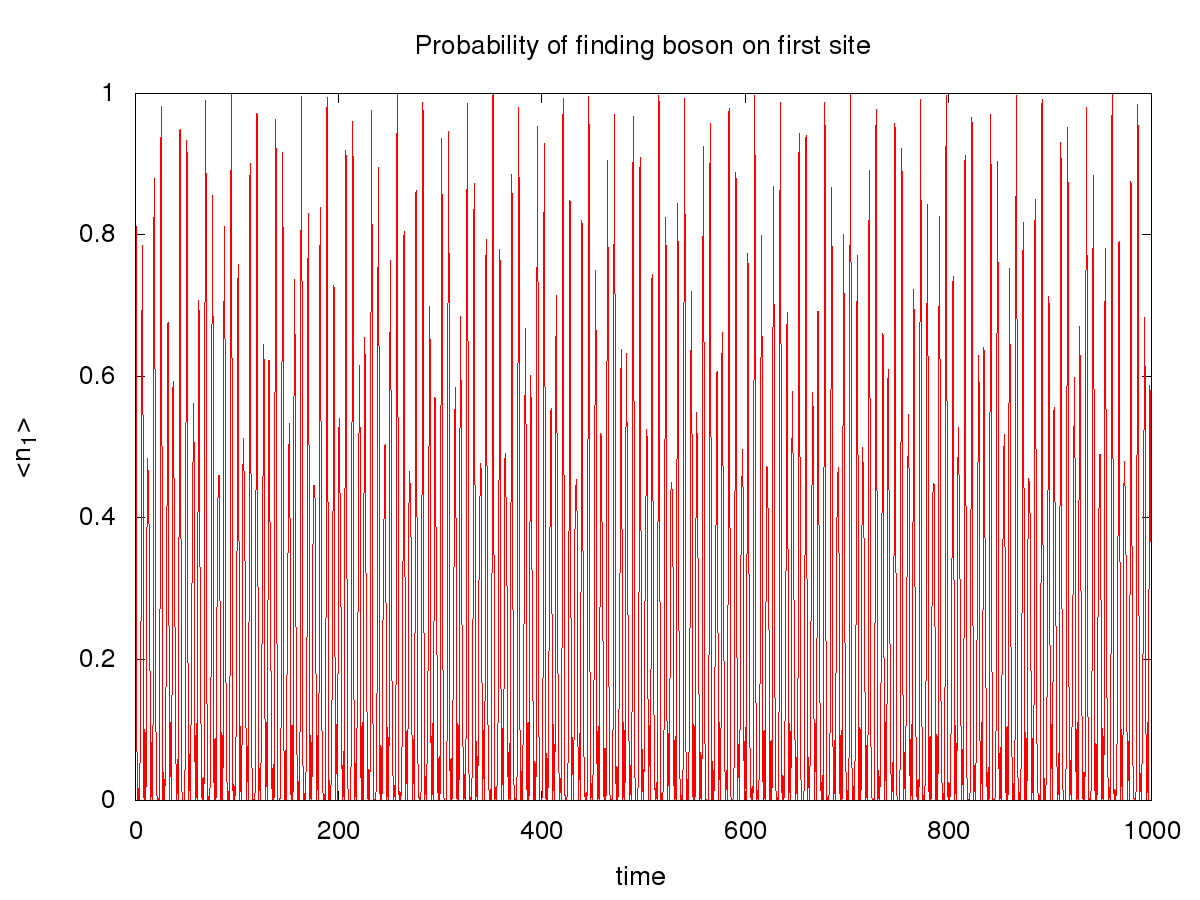
\includegraphics[width=0.9\textwidth]{5_by_1_T1e4_U0}
\end{figure}
\todo{make this full text width if can without adding extra page}
Judging the figure above by eye, it may appear that we have exact revival, but
this is not actually the case. If we look at how long it takes for the system to
get within $\epsilon$ of its initial state (i.e. $\norm{\ket{\psi(t)} -
\ket{\psi(0)}} < \epsilon$) we get the graph below. Note that $t^*$ denotes the
time at which the system got within a particular value of $\epsilon$ of the
initial state.
\begin{figure}[H]
 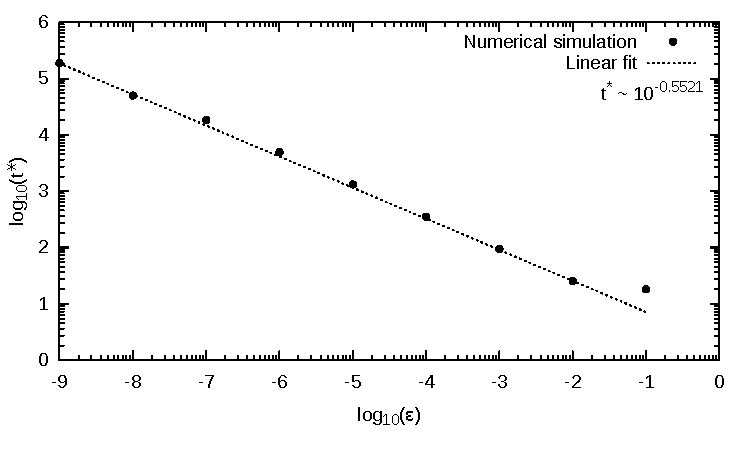
\includegraphics[width=1.0\textwidth]{recurrence_times}
 \centering
\end{figure}
While we see that the system does appear to get arbitrarily close to revival,
but it can take arbitrarily long to do so. This result can be explained in terms
of the Poincar\'e recurrence theorem.


\section{The Poincar\'e Recurrence Theorem}

In 1890, Henri Poincar\'e proved the following theorem for classical mechanics:
\begin{quote}
    Any phase-space configuration $(q, p)$ of a system enclosed in a finite
    volume will be repeated as accurately as one wishes after a finite (be it
    possibly very long) interval of time.
\end{quote}
This theorem was extended to quantum systems in 1956 by P. Bocchieri and A.
Loinger \cite{Bocchieri1957}, where they gave a slightly different form:
\begin{quote}
    Let us consider a system with discrete energy eigenvalues $E_{n}$; if
    $\Psi(t_{0})$ is its state vector in the Schr{\"o}dinger picture at the time
    $t_{0}$ and $\epsilon$ is any positive number, at least one time $T$ will
    exist such that the norm $\norm{\Psi(T) - \Psi(t_0)}$ of the vector $\Psi(T)
    - \Psi(t_{0})$ is smaller than $\epsilon$.
\end{quote}


\subsection{Proof}

The proof presented by Bocchieri and Loinger shows the theorem to be true for an infinite-dimensional system. In this dissertation, we investigate only finite-dimensional systems, and a simpler version of
the proof can be constructed. We will first show that there exists a time $T$ at which $||\ket{\psi(T)}-\ket{\psi(t_0)}||^2<2\epsilon'$ for any $\epsilon'>0$ and then extend this to $||\ket{\psi(T)}-\ket{\psi(t_0)}||<\epsilon$. Note that in
the following we will introduce the notation $\tau=T-t_0$ and $\alpha^2(T)=||\ket{\psi(T)}-\ket{\psi(t_0)}||^2$.

\begin{align*}
 \alpha^2(T)
 &= \left(\bra {\psi(T)}-\bra {\psi(t_0)}\right)\left(\ket{\psi(T)}-\ket{\psi(t_0)}\right)
 \\
 &= 2-\braket{\psi(T)|\psi(t_0)}-\braket{\psi(t_0)|\psi(T)}
 \\
 &= 2-\sum_{j,n=1}^{\mathcal{D}}c_n^* c_je^{iE_{n}T}e^{-iE_{j}t_{0}}\braket{E_n|E_j}-\sum_{j,n=1}^{\mathcal{D}}c_j^*c_ne^{iE_{j}t_{0}}e^{-iE_{n}T}\braket{E_j|E_n}
 \\
 &= 2 - \sum_{n=1}^\mathcal{D} |c_n|^2 e^{iE_{n}(T-t_0)} - \sum_{n=1}^\mathcal{D} |c_n|^2 e^{-iE_{n}(T-t_0)} \ \ \ \text{since} \braket{E_j|E_n}=\delta_{ij}
 \\
 &= 2 \sum_{n=1}^\mathcal{D} |c_n|^2\left(1-\cos\left(E_{n}\tau\right) \right) \ \ \text{because}  \ \sum_{n=1}^\mathcal{D} |c_n|^2=1
 \\
 &\leq 2\sum_{n=1}^\mathcal{D}\left(1-\cos\left(E_{n}\tau\right) \right)
\end{align*}

It is sufficient to show that there is a $\tau$ such that
$\sum_{n=1}^\mathcal{D}{\left(1 - \cos{(E_{n}\tau)} \right)} < \epsilon'$.
This is actually the case according to a standard result of the theory of the
almost-periodic functions.\todo{need reference! The one from Bocchieri is in
German.}

Evidently, if we know that there exists a time $T$ such that
\begin{equation}
    \sum_{n=1}^{\mathcal{D}}%
        {\left ( 1 - \cos{\left(E_{n}\tau\right)} \right )}
    < \epsilon',
\end{equation}
then at this same time $\alpha^{2}(T) < 2 \epsilon'$, which implies $\alpha(T) =
\norm{\ket{\psi(T)} - \ket{\psi(t_0)}} < \sqrt{2 \epsilon'}$. Taking $\epsilon =
\sqrt{2 \epsilon'}$ shows that $\norm{\ket{\psi(T)} - \ket{\psi(t_0)}}$ is
guaranteed be arbitrarily small at some arbitrarily large time $T$.
\todo{is there a problem with using T here and t* elsewhere?}


\section{Large 1D systems}

To determine the mutual rationality or mutual irrationality of the spectrum for
an arbitrarily large one-dimensional system with a single particle, we look to a
result about the eigenvalues of tridiagonal matrices proven by W. Yueh
\cite{Yueh2006}. A tridiagonal matrix has the form
\begin{equation}
    A_{N \times N}
    =
    \begin{pmatrix}
             b &      c &     0  &      0 &  \dots & 0 \\
             a &      b &     c  &      0 &  \dots & 0 \\
             0 &      a &     b  &      c &  \dots & 0 \\
             0 &      0 &     a  &      b &  \dots & 0 \\
        \vdots & \vdots & \vdots & \vdots & \ddots & c \\
             0 &      0 &     0  &      0 &      a & b
    \end{pmatrix}.
\end{equation}
It was shown that the eigenvalues of a matrix of this form are given by
\begin{equation}
    \lambda_{k} = -b + 2 \sqrt{ac} \cos{\!\left( \frac{k \pi}{N+1} \right )}
\end{equation}
where $k=1$, 2,\dots, $N$. The Hamiltonian of any one-dimensional system with
$N$ sites and a single particle has exactly this form, namely
\begin{equation}
    \hat{H}_{N}
    =
    \begin{pmatrix}
         0 &     -J &     0  &      0 &  \dots &  0 \\
        -J &      0 &    -J  &      0 &  \dots &  0 \\
         0 &     -J &     0  &     -J &  \dots &  0 \\
         0 &      0 &    -J  &      0 &  \dots &  0 \\
    \vdots & \vdots & \vdots & \vdots & \ddots & -J \\
         0 &      0 &     0  &      0 &     -J &  0
    \end{pmatrix},
\end{equation}
and consequently has eigenvalues ($k=1$, 2, \dots, $N$.)
\begin{equation}
    \label{1D_eigenvalues}
    E_{k} = 2 J \cos{\!\left( \frac{k \pi}{N+1} \right)}.
\end{equation}
This result is particularly interesting when combined with Niven's theorem
\cite{DoubleIvan}.

\begin{theorem}[Niven's theorem]
    BLA BLA
\end{theorem}
In other word this theorem tells us that if $x$ is rational \textit{in degrees},
then the only possible rational values of $\cos(x)$ are $0, \pm \frac{1}{2}$ and
$\pm 1$. Note in our case that $\frac{k\pi}{N+1}\neq 0, \pi$ for $k=1$, 2,
\dots, $N$, so $\cos{\!(\frac{k\pi}{N+1})} \neq \pm 1$ and we are left with 3
rational options.

When we are evaluating in degrees, equation \eqref{1D_eigenvalues} becomes
\begin{equation}
    E_{k} = 2 J \cos{\!\left ( \frac{180k}{N+1} \right )}.
\end{equation}
The argument of cosine here is clearly rational since $N$ and $k$ are integers.
Hence we know that for a system with non-degenerate eigenvalues, there can be at
most 3 eigenvalues, $\lbrace 0, \pm \frac{J}{2} \rbrace$, that are rational. So
$\mathcal{D} \leq 3$ for a system with all eigenvalues rational (the lattice
must have at most 3 sites). We must have at least $(N-3)$ irrational eigenvalues
for any larger system size. \todo{Can I prove that all systems larger than N=3
have **mutually** irrational eigenvalues?}


\newpage
\bibliographystyle{plain}
\bibliography{honours}


%Note: \url{https://arxiv.org/pdf/1007.5331.pdf} has a good description of what quantum ergodicity is on page 10
%\\ Note: \url{http://www.physicspages.com/tag/field-operators/} was the thing that made field operators make some sense for me
%\\Note: \url{http://www.nucleares.unam.mx/~alberto/apuntes/altland.pdf} was super useful for background second quantisation.
%\\Note: \url{http://iopscience.iop.org/article/10.1209/epl/i2004-10265-7/pdf} mentions finding the 1D B-H model to not be integrable. This could be v useful when including U(n*n-n) term
%\\Note: \url{https://arxiv.org/pdf/cond-mat/0410614v1.pdf} might have good stuff for background section of dissertation
%\newpage


%\section{Additional questions for Danny}




\end{document}